\documentclass[oneside,12pt,a4paper]{book}	

% ---------------------------------------------------
% Preambulum
% ---------------------------------------------------

\usepackage[magyar,english]{babel}
\usepackage[utf8]{inputenc}
\usepackage{t1enc}
\usepackage{indentfirst}
\usepackage{graphicx}
\usepackage{amsmath}
\usepackage{amsfonts}
\usepackage{url}
\usepackage{algorithmic}
\usepackage{algorithm}
\usepackage{mdwlist}
\usepackage{listings}
\usepackage{wrapfig}
\usepackage{epigraph}
\lstset{basicstyle=\footnotesize\ttfamily}
\newcommand{\inlinecode}{\texttt}
\DeclareGraphicsExtensions{.png,.jpg}
\usepackage[left=3.5cm,right=2.5cm,top=2.5cm,bottom=2.5cm]{geometry}
\linespread{1.3}

\usepackage{tikz}

\newcounter{treeline}

\newcommand{\treeroot}[1]{% Title
\node[above] at (0,0) {#1};%
\setcounter{treeline}{0}
}

\newcommand{\treeentry}[2]{% Title, Level
\draw[->] (#2-1,-\value{treeline}/2) -- (#2-1,-\value{treeline}/2-0.5) -- (#2+0.5,-\value{treeline}/2-0.5) node[right] {#1};
\stepcounter{treeline}
}

\newcommand{\altentry}[2]{% Title, Level
\draw[->] (#2-1,-\value{treeline}/2) -- (#2-1,-\value{treeline}/2-0.5) -- (#2+0.5,-\value{treeline}/2-0.5) node[right] {#1};
\foreach \x in {1,...,#2}
{   \draw (\x-1,-\value{treeline}/2) -- (\x-1,-\value{treeline}/2-0.5);
}
\stepcounter{treeline}
}

\DeclareMathOperator{\diag}{diag}
\setcounter{secnumdepth}{3}
\setcounter{tocdepth}{3}

\begin{document}
\clearpage
\thispagestyle{empty}
\hspace{-10pt}\begin{tabular}{p{3cm} p{1cm} p{10cm}}
\raisebox{-2.5cm}{
\includegraphics[scale=0.2]{ELTE_logo}} & &
\large{\foreignlanguage{magyar}{Eötvös Loránd Tudományegyetem\newline Informatikai Kar\newline
 Programozási Nyelvek és \newline Fordítóprogramok Tanszék}}
\end{tabular}
\vspace{0.4cm}
\hrule
\vspace{6cm}
\begin{center}
\LARGE{\textbf{Applying slicing algorithms on large code bases}}
\end{center}
\vspace{3cm}
\begin{tabular}{p{7cm} p{8cm}}
\large{Tibor Brunner \vspace{5pt} \newline doktorandusz} &
\large{\foreignlanguage{magyar}{ Olivér Hechtl \vspace{5pt} \newline programtervező informatikus MSc}}
\end{tabular}\vspace{6cm}
\begin{center}
\large{Budapest, 2017}
\end{center}
\newpage
\setcounter{page}{1}
\pagenumbering{arabic}
\pagestyle{plain}
\tableofcontents

\chapter{Introduction}
\epigraph{Everyone knows that debugging is twice as hard as writing a program in the first place. So if you're as clever as you can be when you write it, how will you ever debug it?}{\textit{Brian Kernighan}}

Nowadays, there are a lot of tools available for debugging. A developer can examine call stacks, variable informations, and so on. There are a lot of times when a bug is when some variable does not behave like the writer of that code part would expect. When the programmer discovers it, he must follow back the path of assignments, and find out where did it get an unexpected value. Program slicing targets this kind of debugging. We can define a program slice as a part of the program which contains a selected statement, and all other statements which influences it, or gets influenced by it. These two types are respectively called backward and forward slicing. Basically this is what many programmers do intuitively, when facing with bugs. In this thesis, I'll introduce a few approaches for computing slices, and describe a working prototype tool application, which can analyze C++ programs, and compute slices of them. I've used the help of the Clang/LLVM compiler infrastructure, which builds the AST of the program and provides an interface to analyse it using C++.

\chapter{Slicing, methods and efficiency}
\section{About slicing}
For better understanding programs, programmers organize code into structures. They write sub-problems into functions, and organize variables and data to structs. Also, with object oriented design, they put these into classes. These are all good for separating the data, and the procedures on data. But these are not helpful when we need to examine a flow of data in the program. Slicing gets useful in this scenario. This is a program analysis technique introduced by Mark Weiser\cite{weiser84}. In his paper, he wrote: ``Program slicing is a decomposition based on data flow and control flow analysis''. We define slicing as a subset of the program, which only includes the statements which have transitive control or data dependency regarding the selected statement. 

\section{Types of slicing}
There is two different type of slicing known: static and dynamic. While dynamic slicing gets the statements which could affect the selected statement at a particular execution of the program with a fixed input, static slicing examines it statically, including all possible statements which could affect that selected statement. In this thesis, I'll focus on static slicing methods. There are two different subtypes of static slicing, backward and forward. They are indicating the relevant statements' direction from our selected statement. 

\section{Methods for slicing}
We can construct slices via various methods on different representations of the program. All of these are using some kind of graph structures, which can be traversed through for searching the transitive data dependences.

\subsection{Dependences}
Before I describe the various methods currently available for slicing, we must get to know what dependences in programs are. There are two kinds of dependences: control and data. They can be defined by the control flow graph (CFG) of the program. Given the following example:

\begin{lstlisting}[language=C++]
int main(){
  int sum = 0;
  int i = sum;
  while (i < 11){
    sum += i;
    i++;
  }
}
\end{lstlisting}

\begin{wrapfigure}{r}{0.4\textwidth}
  \centering
    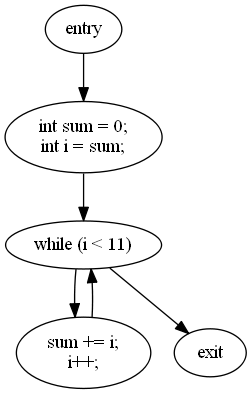
\includegraphics[width=0.38\textwidth]{horwitz_cfg.png}
  \caption{Control-flow graph}
  \label{fig:horwitz_cfg}
\end{wrapfigure}

It's control-flow graph can be seen on \ref{fig:horwitz_cfg}. This type of graph is created from the program by grouping the statements into basic blocks. Each basic block consists a maximal amount of consecutive statements without any jumps. In a high-level language, such as C++, a jump can be either a branch statement, like an \texttt{if} and a \texttt{switch-case}, or a loop statement, like a \texttt{while}. In the example, we can see that it's CFG consists three basic blocks, and two special blocks, namely \texttt{entry} and \texttt{exit}, which represent the entry and exit points of the program, respectively.

Therefore, control dependence can be defined in the knowing of post-dominance. As written in \cite{slicing-survey}:

"A node \textit{i} in th CFG is \textit{post-dominated} by a node by \textit{j} if all paths from \textit{i} to STOP pass through \textit{j}. A node \textit{j} is \textit{control dependent} on a node \textit{i} if (i) there exists a path \textit{P} from \textit{i} to \textit{j} such that \textit{j} post-dominates every node in \textit{P}, excluding \textit{i} and \textit{j}, and (ii) is not post-dominated by \textit{j}."

It basically means that every statement under a branch or loop are control dependent of the control statement's predicate. Excluding the unstructured and structured jump statements, \texttt{continue},\texttt{break} and \texttt{goto}, drawing control dependences between statements creates a tree, with the root being the inspected function, and control statements form the branches. I discuss later in detail the control dependences created by structured jumps. 

A data dependence between two statements means that if we change their order, the meaning of the program changes, or becomes ill-formed. There are two types of data dependences: \textit{flow dependences} and \textit{def-order dependences}. According to Horwitz\cite{horwitz-interproc}, we can define these with the following rules:

There is a flow dependence between statement s1 and s2 if:
\begin{enumerate}
  \item s1 defines variable x.
  \item s2 uses x.
  \item There is a path between s1 and s2 in program execution with no intervening definitions of x in between, and s2 can be reached by control from s1. 
\end{enumerate}

Definition in this context means a bit different than usual: it can be either an initial definition of a variable but an assignment where x is on the left side is also counts as a definition. In compiler theory, flow-dependence referred as reaching definition of a variable.

In the presence of loops, there are two further classification of flow-dependence: loop-carried and loop-independent. A flow-dependence is loop-carried if it satisfies all rules above and also:
\begin{enumerate}
  \item includes a backedge to the predicate of the loop.
  \item s1 and s2 are enclosed in the loop.
\end{enumerate}

Backedge means that there is a flow dependence between the statement and the predicate of the loop, therefore the loop uses the variable which that statement defines. In the example above, the statement \texttt{i++} is like this.

Loop-independent flow-dependences can be described as the common ones which has no backedge to the loop predicate. 

On the other hand, def-order dependence between statement s1 and s2 is different from loop-independent flow-dependences only in that s2 instead of using x, it also defines it. The other two rules stays the same. 

These definitions are used in all slicing methods, but differently. I will elaborate these in each section.

\subsection{Data flow equations}
This method is created by Mark Weiser. It is based on the analysis of the CFG. As he wrote in \cite{weiser84}, he defines a slice regarding a \textit{slicing criterion}, which consists of a pair \textit{(n, V)} where n is a statement of the program and V is a subset of the program's variables, which we are slicing on. He also writes that a slice of a program is an executable, which has only the relevant statements in it.

To calculate which statements should be included in the slice, he defines two sets of variables: \textit{directly} and \textit{indirectly relevant} variables. As written in \cite{slicing-survey}, he provides the following equations for them:

For determining \textit{directly} relevant variables and statements:
% TODO beautify

For each edge $i \rightarrow_{CFG} j$ in the CFG:
\begin{align*}
R^0_C(i) &= R^0_C(i) \cup \{ v | v \in R^0_C(j), v \notin \textsc{Def}(i) \} \cup \{ v | v \in \textsc{Ref}(i), \textsc{Def}(i) \cap R^0_C(j) \neq \emptyset \} \\
S^0_C &= \{ i | (\textsc{Def}(i) \cap R^0_C(j) \neq \emptyset, i \rightarrow_{CFG} j \}
\end{align*}

And for determining \textit{indirectly} relevant variables and statements:
\begin{align*}
B^k_C &= \{ b | \exists i \in S^k_C, i \in \textsc{Infl}(b) \} \\
R^{k+1}_C(i) &= R^k_C(i) \cup \bigcup_{b \in B^k_C} R^0_{(b, \textsc{Ref}(b))} (i) \ \\
S^{k+1}_C &= B^k_C \cup \{ \textsc{Def}(i) \cap R^{k+1}_C(j) \neq \emptyset, i \rightarrow_{CFG} j \} 
\end{align*}

He also says that a slice is statement-minimal if it couldn't have less statements. The slice then is computed in two steps:
First by determining \textit{directly} relevant variables by the equation above. In it, $\textsc{Def}(i)$ and $\textsc{Ref}(i)$ means the variables that statement $i$ defines or uses, respectively. $R^0_C(i)$ will contain the directly relevant variables of statement $i$. It is an iterative process, and starts with the values in the slicing criterion: $R^0_C(n) = V$, and for all other sets initialized as $\emptyset$. 
% TODO walk through the example.

\subsection{Information flow relations}
\subsection{PDG based graph reachability}


\chapter{LLVM/Clang infrastructure}
\section{About Clang}
\section{The Clang AST}
\section{AST Matchers}

\chapter{Implementation and algorithm}
\section{The approach}
\section{Building the PDG}
\subsection{Control dependences}
\subsection{Data dependences}

\section{Implementing slicing}


\addcontentsline{toc}{chapter}{Glossary}
\begin{thebibliography}{Textttext}
\bibitem{weiser84}
  M. Weiser,
  Program slicing,
  IEEE Transactions on Software Engineering,
  10(4):352-357,
  1984.

\bibitem{slicing-survey}
  Tip, Frank,
  A survey of program slicing techniques,
  Journal of programming languages 3.3,
  121-189,
  1995. 

\bibitem{horwitz-interproc}
  Horwitz, Susan, Thomas Reps, and David Binkley,
  Interprocedural slicing using dependence graphs, 
  ACM Transactions on Programming Languages and Systems,
  (TOPLAS) 12.1: 26-60,
  1990.

\end{thebibliography}

\end{document}